% =====================================================================================
%  Revised sections for "A Systematic Review and Comparative Analysis of Arabic-Centric
%  SOTA Language Models" (Systematic_revised_1).
%
%  Each block below is a drop-in replacement for the passage named in its header.
%  Every number is recomputed from the as-run artifacts by audit/audit_track_b.py
%  (see ../AUDIT_REPORT.md). Figures: figures/fig_trackb_status.pdf (new Fig. 2) and
%  figures/fig_trackb_vs_baseline.pdf (new Fig. 3).
%
%  Arabic script (Appendix B) needs XeLaTeX or LuaLaTeX. In the IEEE Access template add:
%      \usepackage{fontspec}
%      \newfontfamily\arabicfont[Script=Arabic]{Amiri}   % or any installed Arabic font
%      \newcommand{\ar}[1]{\bgroup\textdir TRT\arabicfont #1\egroup}   % LuaLaTeX
%  or with XeLaTeX + polyglossia: \setotherlanguage{arabic} and \newcommand{\ar}[1]{\textarabic{#1}}.
%  If you must stay on pdfLaTeX, replace \ar{...} by a transliteration.
%  Citation keys \cite{qwen25} and \cite{falconarabic} stand for references [13] and [10]
%  of the submitted manuscript; rename them to your .bib keys.
% =====================================================================================

%% ------------------------------------------------------------------------------------
%% ABSTRACT — replace the sentences from "We reveal the presence of a confound" to
%% "...from significantly better than random to zero."
%% ------------------------------------------------------------------------------------
We reveal a confound that per-paper reading of results cannot expose: under one fixed
zero-shot harness, most decoder scores are not capability measurements at all. An audit
of the harness against its own logged artifacts shows that 21 of the 23 completed decoder
runs are determined by silent harness defects---gold labels that are missing from the
prepared data or never resolved, prompts that omit the answer options or the question,
and degenerate generations that a permissive answer extractor converts into valid-looking
option letters---and that every affected cell is at or below the accuracy of always
answering the same letter. Only two cells carry evidence of capability (ALLaM-7B and
Qwen2.5-7B on EXAMS AR: 53.4\% and 49.0\% against a 26.3\% constant-letter baseline).
Because defective cells enter leaderboard averages as ordinary numbers, single-number
leaderboards rank harness behavior rather than models. We fine-tune two compact encoders
(MARBERT, AraBERT) on five Arabic understanding datasets and evaluate four
instruction-tuned decoders (ALLaM, JAIS, Qwen, Falcon) zero-shot under 4-bit quantization
or CPU offloading, and we release an artifact-only audit that flags such cells by
comparing each score with constant-letter baselines, gold-label coverage, and
prompt-field coverage.

%% ------------------------------------------------------------------------------------
%% INTRODUCTION — contribution 2 (replace item 2 of the contribution list)
%% ------------------------------------------------------------------------------------
\item An audit showing that, in a single fixed zero-shot harness, low and zero decoder
      scores were produced by harness defects (missing or unresolved gold labels,
      prompts missing options or stems, and degenerate outputs admitted by a permissive
      extractor) rather than by model capability, and that naive leaderboard averaging
      therefore misranks the generative models. The as-run extractor, the logged raw
      generations, and the audit are given in Appendices A and B so that the reader can
      verify this claim.

%% ------------------------------------------------------------------------------------
%% SECTION VI-A (Experimental Setup) — replace the paragraph beginning
%% "Track B (decoder zero-shot)." with the following two paragraphs.
%% ------------------------------------------------------------------------------------
\textbf{Track B (decoder zero-shot).} Four accessible instruction-tuned decoders were
evaluated zero-shot: ALLaM-7B-Instruct, Jais-13B-chat, Qwen2.5-7B-Instruct~\cite{qwen25}
(a strong multilingual baseline), and Falcon-7B-Instruct. To fit the 8~GB budget, the
7B models were loaded in 4-bit NF4 quantization (double quantization, fp16 compute
dtype); Jais-13B was instead run in fp16 with CPU offloading, as 4-bit offload proved
unstable on our stack. Prompts were plain text (no chat template) in the format
``\emph{Question} / lettered options / \emph{choose the correct answer; answer with one
letter only} / \emph{Answer:}'', truncated to 1,024 tokens. Decoding was greedy
(\texttt{do\_sample=False}) with a 20-token budget for ALLaM, Qwen, and Falcon; the
Jais configuration used a budget of a single token (\texttt{max\_new\_tokens=1}). The predicted option was
recovered by the rule-based extractor reproduced verbatim in Appendix~A. Track~B covered
six multiple-choice benchmarks across three families: commonsense/STEM (Arabic MMLU,
$n{=}14{,}455$; EXAMS AR, $n{=}537$; Madinah QA, Arabic Language General and Grammar,
$n{=}977$), cultural understanding (ArabCulture and AraDiCE-Culture, Jordan, Palestine,
Lebanon, and Syria subsets, $n{=}1{,}097$ and $n{=}120$), and social/safety meaning
(AraTrust, $n{=}522$, three options per item). We report accuracy. Table~IV summarizes
the configuration.

\textbf{Provenance.} All runs used the same prepared data (created once, before any
evaluation). The ALLaM and Qwen result files were produced on 4--6~April~2026 by an
earlier revision of the evaluation script that was not preserved; Jais (21--22~April)
and Falcon (30~May, a rerun after a cache-API fix) used the surviving revision. Only the
Falcon rerun logged raw generations, and only for the first five items of each dataset;
for ALLaM, Jais, and Qwen no raw generations survive. We state below which conclusions
rest on logged outputs and which on the result files alone.

%% ------------------------------------------------------------------------------------
%% SECTION VI-A — Track A paragraph: append after
%% "...so any score difference reflects the model rather than the optimization schedule."
%% ------------------------------------------------------------------------------------
Two properties of this protocol bound the interpretation of Track~A. First, the
checkpoint reported for each run is the best of the three epochs as measured on the
test split (\texttt{load\_best\_model\_at\_end} with the test split as evaluation set),
so the reported scores are mildly optimistic; the released code selects on a
validation split carved from the training data instead. Second, ANERcorp, which is
distributed one word per row, was run as context-free word-level tag classification
(each word classified in isolation over the nine BIO tags), not as sentence-level NER;
its macro-F$_1$ is therefore not comparable to the entity-level F$_1$ reported in the
NER literature.

%% ------------------------------------------------------------------------------------
%% SECTION VI-B — replace the sentence
%% "AraBERT, pretrained on news with explicit clitic segmentation, leads on NER
%%  (ANERcorp, 54.7 vs. 53.0), the most MSA-like and boundary-sensitive task."
%% ------------------------------------------------------------------------------------
AraBERT, pretrained on news with explicit clitic segmentation, leads on the word-level
ANERcorp tagging task (54.7 vs.\ 53.0), the most MSA-like of the five datasets; because
words are classified without sentence context, this comparison reflects lexical rather
than boundary-sensitive NER ability.

%% ------------------------------------------------------------------------------------
%% SECTION VI-C — replace the whole subsection (title, text, Fig. 2, Fig. 3).
%% ------------------------------------------------------------------------------------
\subsection{Track B: Zero-Shot Decoders and Silent Harness Defects}

Fig.~\ref{fig:trackb-status} reports the full grid of zero-shot outcomes together with
the result of auditing each cell. The audit uses only the artifacts of the original
runs: the prepared data, the as-run prompt builders, gold-label lookup and extractor,
the result files, and the logged Falcon generations. For every cell it computes the
share of items whose gold label the as-run code resolves, whether the prompt shows the
question, the context, and the options, the chance level, and the accuracy of each
\emph{constant-letter predictor} (always answering A, always B, \ldots), and it tests the
reported accuracy against the best constant-letter baseline with a one-sided exact
binomial test.

\begin{figure*}[t]
  \centering
  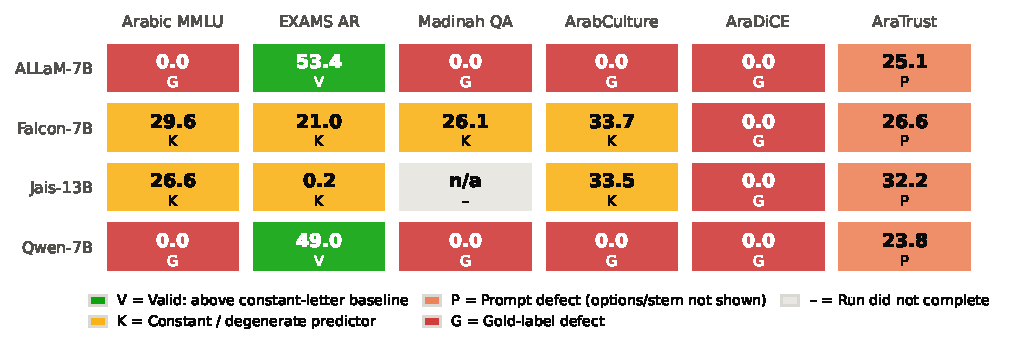
\includegraphics[width=\textwidth]{figures/fig_trackb_status.pdf}
  \caption{Track~B: reported zero-shot accuracy (\%) of four accessible instruct
  decoders under one fixed harness on an 8~GB GPU, annotated with the audit status of
  each cell. V: significantly above the best constant-letter baseline
  ($p<10^{-28}$). K: indistinguishable from, or below, a constant-letter predictor.
  P: the prompt omitted the answer options (AraTrust). G: gold-label defect (no gold
  column, AraDiCE; or exactly 0.0\% although the gold resolves for every item).
  --: no result file was produced. Only the two V cells are capability measurements.}
  \label{fig:trackb-status}
\end{figure*}

Four distinct defects account for 21 of the 23 completed runs.

\emph{(i) Missing gold labels (AraDiCE).} The prepared AraDiCE-Culture data contains
only the columns \texttt{QID}, \texttt{Question}, \texttt{Option A}, \texttt{Option B},
and \texttt{Option C}; the dataset ships no answer column. The official
lm-evaluation-harness task fixes the target to the first option
(\texttt{doc\_to\_target: 0}), a convention our harness did not implement. The gold
lookup therefore returned an empty string for all 120 items, no prediction could match,
and every model scored exactly 0.0\%. This zero is a property of the harness, not of
the models, and says nothing about dialectal ability.

\emph{(ii) Unresolved gold labels (ALLaM and Qwen).} ALLaM-7B and Qwen-7B score exactly
0.0\% on Arabic MMLU (14,455 items), Madinah QA (977), and ArabCulture (1,097), yet
53.4\% and 49.0\% on EXAMS AR. Under the surviving code this outcome is not reachable:
the gold label resolves for 100\% of these items, and the extractor maps almost any
Arabic string to an option letter (Appendix~A), so even a model answering at random
would score near chance. The zeros coincide exactly with the gold-label field names:
the three datasets store their answer in \texttt{Answer Key} (Arabic MMLU, Madinah QA)
or a nested \texttt{answer\_key} record (ArabCulture), whereas the two datasets on which
both models score above zero use \texttt{answer} (EXAMS AR) or \texttt{Answer}
(AraTrust). Jais and Falcon, evaluated later with the surviving revision, score
non-zero on all three datasets. The evidence therefore points to a gold lookup in the
unpreserved April revision that did not resolve \texttt{Answer Key} or
\texttt{answer\_key}. Because no raw generations survive for these runs, we treat this
as the most likely explanation rather than a verified one; either way, the zeros are
not capability measurements, and in particular they are not failures to parse verbose
output.

\emph{(iii) Incomplete prompts (AraTrust, ArabCulture, Madinah QA).} The AraTrust prompt
rendered only the question: its three options were never shown, yet responses were
scored against option letters, so all four AraTrust scores (23.8--32.2\%) are below the
best constant-letter baseline (36.6\%) and carry no information. The ArabCulture prompt
builder did not recognize the field holding the scenario sentence
(\texttt{first\_statement}), so all 1,097 prompts consist of an empty question followed
by three completions; 602 of the 977 Madinah QA prompts and 706 of the Arabic MMLU prompts
omit the reading passage stored in the \texttt{Context} field.

\emph{(iv) Degenerate outputs admitted by a permissive extractor (Falcon, Jais).} Every
logged Falcon generation is a single character repeated to the token limit, for example
\ar{ألللللللللللللللللل} (\emph{alif} followed by a run of \emph{lam}) on 24 of the 30 logged
items (Appendix~B). The extractor's first rule maps any string that begins with
\emph{alif} to option A, so 25 of the 30 logged degenerate outputs became the prediction
``A''. Falcon's accuracies are accordingly at or below the always-A baseline on every
dataset (Arabic MMLU 29.6 vs.\ 31.2\%, Madinah QA 26.1 vs.\ 26.7\%, EXAMS AR 21.0 vs.\
23.6\%, ArabCulture 33.7 vs.\ 34.1\%). For Jais, which generated a single token, the
number of correct Arabic MMLU answers (3,846) equals exactly the number of items whose
gold answer is B, and the same holds for AraTrust (168); its ArabCulture score (367
correct) lies within four items of the always-B count (371). Jais therefore behaved as
an (almost) constant ``B'' predictor, and its near-zero EXAMS AR score (1 of 537) is
equally uninformative. These cells look like ordinary, above-zero measurements, but
what they record is the answer-letter distribution of each benchmark.

\begin{figure}[t]
  \centering
  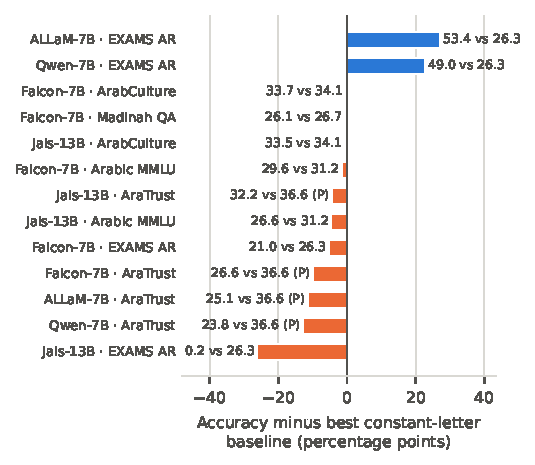
\includegraphics[width=\columnwidth]{figures/fig_trackb_vs_baseline.pdf}
  \caption{Every non-zero Track~B score with a resolvable gold label, expressed as its
  difference from the best constant-letter baseline of the same benchmark (labels:
  reported vs.\ baseline accuracy, \%; P marks prompts that omitted the options). Only
  ALLaM-7B and Qwen-7B on EXAMS AR exceed the accuracy of always answering one letter.}
  \label{fig:trackb-vs-baseline}
\end{figure}

Fig.~\ref{fig:trackb-vs-baseline} makes the consequence explicit. Of the thirteen
non-zero scores with a resolvable gold label, eleven do not exceed the best
constant-letter baseline; the two that do, ALLaM-7B (53.4\%, $p<10^{-39}$) and
Qwen-7B (49.0\%, $p<10^{-28}$) on EXAMS AR, are the only Track~B results we regard as
capability measurements. The defects are therefore not failures of the extractor to
find an answer in verbose output (false negatives); where the extractor contributes, it does so by turning meaningless output
into a valid-looking letter (false positives), and the dominant causes of the zeros
lie in the gold labels and the prompts. Jais-13B's Madinah QA run did not complete and
produced no result file; we report it as missing rather than as a score.

%% ------------------------------------------------------------------------------------
%% SECTION VI-D — replace the first paragraph and the numbered list
%% ------------------------------------------------------------------------------------
Collapsing the two tracks into a single ranking places the fine-tuned encoders
(MARBERT 68.2\%, AraBERT 66.8\%) far above every decoder (Falcon 23.0\%, Jais 20.8\%,
ALLaM 14.3\%, Qwen 13.4\% when the Track~B cells are averaged by category as in
Section~VI-B). This ordering is an artifact of three compounding confounds:
\begin{enumerate}
  \item it compares fine-tuned encoders with zero-shot decoders;
  \item it compares discriminative macro-F$_1$ with generative accuracy on different
        tasks; and
  \item it averages Track~B cells that are not measurements (Fig.~\ref{fig:trackb-status})
        as if they were: 21 of the 23 decoder cells entering these averages are gold-label
        defects, prompt defects, or constant-letter predictors.
\end{enumerate}
Each confound alone would distort the ranking; together they determine it. The decoder
ordering is itself an artifact: Falcon and Jais rank above ALLaM and Qwen only because
their degenerate outputs collect the constant-letter share of each benchmark while
ALLaM's and Qwen's cells were zeroed by the gold lookup, although ALLaM and Qwen are the
only decoders with evidence of above-baseline accuracy. This observation motivates the
protocol recommendations of Section~VII.

%% ------------------------------------------------------------------------------------
%% SECTION VI-D — last paragraph: replace the sentence beginning
%% "Likewise, the 'Falcon-7B' run uses the base instruct checkpoint..."
%% ------------------------------------------------------------------------------------
Likewise, the ``Falcon-7B'' run uses the base \texttt{falcon-7b-instruct} checkpoint,
whose pretraining and tokenizer are English-centric, rather than the Falcon-Arabic
system of~\cite{falconarabic}; its degenerate Arabic output (Section~VI-C) says nothing
about Falcon-Arabic. We did not isolate whether the degeneration stems from the
checkpoint, the 4-bit quantization, or the generation path; a one-item control without
batching also produced a malformed single-byte output.

%% ------------------------------------------------------------------------------------
%% SECTION VII — opening paragraph: replace
%% "...even with a single fixed harness the answer-extraction layer alone can move a
%%  model's apparent score from well above chance to zero."
%% ------------------------------------------------------------------------------------
Our empirical study sharpens this concern, since even within a single fixed harness,
defects in gold-label handling, prompt construction, and answer extraction produced
scores that were indistinguishable from real measurements and that decided the ranking.

%% ------------------------------------------------------------------------------------
%% SECTION VII-C — replace the whole subsection
%% ------------------------------------------------------------------------------------
\subsection{Defect-Robust Scoring}
Section~VI shows that a zero-shot harness can fail silently at three points---the gold
label, the prompt, and the extractor---without any indication in the reported score.
We add five requirements that current protocols typically omit.
\begin{enumerate}
  \item Multiple-choice items should be scored by log-likelihood comparison over the
        candidate options (rank classification) rather than by generation and letter
        parsing; this removes the extractor entirely for closed-form questions.
  \item The harness must resolve a gold label for every item through an explicit,
        per-dataset schema and must abort, not score, when it cannot. A benchmark
        without an answer column (e.g., AraDiCE-Culture) needs its documented target
        convention, and options must then be shuffled so that the gold position varies.
  \item Every score must be reported next to its chance level and its best
        constant-letter baseline, together with the distribution of predicted letters.
        A score at or below the constant-letter baseline, or a prediction distribution
        concentrated on one letter, indicates a defect, not a capability.
  \item When free-form generation is unavoidable, the extractor must have an explicit
        ``unparsed'' outcome, accept only option labels that were actually shown, and
        reject degenerate output; the parse rate must be reported alongside accuracy.
  \item Evaluations should log every raw generation and the exact prompt, and check
        before any GPU time is spent that each prompt contains the question, the
        context, and all options (Appendix~B).
\end{enumerate}
Applied to the artifacts of our runs, requirements 2--5 flag every defective cell in
Fig.~\ref{fig:trackb-status}; the released audit implements them without rerunning any
model, and the released harness implements all five.

%% ------------------------------------------------------------------------------------
%% SECTION VIII — replace the sentence
%% "Specifically, the answer extraction issue described above is extremely relevant to
%%  automated assessment."
%% ------------------------------------------------------------------------------------
Specifically, the scoring defects described above are directly relevant to automated
assessment: a grader can mark a correct answer wrong, and it can also accept a
meaningless response as a valid answer, which is the more dangerous failure in a
tutoring context.

%% ------------------------------------------------------------------------------------
%% SECTION IX — replace the paragraph "Measurement as a variable."
%% ------------------------------------------------------------------------------------
\textbf{Measurement as a variable.} The main takeaway from our experiments is that, in
the zero-shot regime, the evaluation harness can determine the score more than the model
itself: the same ALLaM checkpoint scores 53.4\% on EXAMS AR and exactly 0.0\% on Arabic
MMLU because of how the gold label was looked up, and a model emitting a repeated
character scores within a point of a genuine-looking 30\%. Comparisons of scores across
papers therefore become questionable: a good score reported by a vendor and a bad score
reported by a third party could differ only in the harness. Constant-letter baselines,
gold-coverage checks, reported parse rates, and likelihood-based scoring
(Section~VII) are required steps for meaningful evaluation.

%% ------------------------------------------------------------------------------------
%% SECTION X (Conclusion) — replace the sentences from "the study contributes the
%% paper's central finding:" to "...that current protocols typically omit."
%% ------------------------------------------------------------------------------------
the study contributes the paper's central finding: under a unified zero-shot harness,
21 of 23 decoder scores were produced by silent harness defects---missing or unresolved
gold labels, prompts without options or stems, and degenerate outputs converted into
option letters---and naive leaderboard averaging consequently misranks the models.
This finding gives empirical support to the long-standing call for standardized Arabic
evaluation and adds concrete requirements that current protocols typically omit:
explicit gold-label schemas, constant-letter baselines, prompt-coverage checks, and
likelihood-based scoring with reported parse rates.

%% ------------------------------------------------------------------------------------
%% APPENDIX A — replace the whole appendix (and delete footnote 1)
%% ------------------------------------------------------------------------------------
\section*{Appendix A\\As-Run Answer Extraction and Gold-Label Logic}

The Track~B scores in Fig.~\ref{fig:trackb-status} were produced by the following
procedure, transcribed from the evaluation code. For each item the model generates up
to the configured budget (20 tokens; 1 for Jais), and the new tokens are decoded to a
string $g$. The prediction is obtained as follows, in order:
\begin{enumerate}
  \item \emph{Strip.} $t \leftarrow \mathrm{strip}(g)$.
  \item \emph{Arabic leading character.} If $t$ begins with \ar{أ} or \ar{ا}
        (\emph{alif}), return A; with \ar{ب} return B; with \ar{ج} C; with \ar{د} D;
        with \ar{هـ} or \ar{ه} E. The test is on the first character only, so any Arabic
        word beginning with one of these letters is mapped to a letter---for example
        \ar{الإجابة} (``the answer'') to A and \ar{بناءً} (``based on'') to B.
  \item \emph{Latin leading character.} Else, if $\mathrm{upper}(t)$ begins with A, B,
        C, D, or E, return that letter (so ``Because\ldots'' becomes B).
  \item \emph{Anywhere search.} Else return the letter mapped from the first occurrence,
        anywhere in $t$, of any character in \{\ar{أ}, \ar{ا}, \ar{ب}, \ar{ج}, \ar{د},
        \ar{ه}, A--E\}; the character class also contains \ar{ھ} (U+06BE) and the
        \emph{tatweel}, which are returned unmapped.
  \item \emph{Digit.} Else, if $t$ begins with a digit 1--5, return A--E.
  \item \emph{Fallback.} Else return the first ten characters of $t$.
\end{enumerate}
There is no extraction-failure state: the procedure always returns a string, and
outputs that reach step~6 are scored as incorrect without being counted or reported.
The gold label is taken from the first non-empty field among \texttt{answer},
\texttt{Answer}, \texttt{Answer Key}, \texttt{answer\_key}, \texttt{correct\_answer},
\texttt{label}, and \texttt{gold} (with nested \texttt{english\_answer\_key}
or \texttt{arabic\_answer\_key} for record-valued fields), mapped to a letter; when no
field is present it returns an empty string, which no prediction can equal. A prediction
counts as correct only if it equals the gold letter exactly.

Because step~2 inspects only the first character and step~4 accepts the most frequent
letters of the Arabic alphabet anywhere in the text, the procedure has almost no false
negatives on Arabic output but many false positives: a degenerate generation beginning
with \emph{alif} is scored as the answer ``A''. The revised harness released with this
paper replaces it by (1)~log-likelihood scoring and (2)~for generation, a strict
extractor that accepts an option label only at the start of the output and followed by
a delimiter (or after an explicit ``the answer is''), only among the options shown,
rejects degenerate repetition, and records all other outputs as unparsed.

%% ------------------------------------------------------------------------------------
%% APPENDIX B — replace the whole appendix (including the "Note to authors")
%% ------------------------------------------------------------------------------------
\section*{Appendix B\\Logged Raw Generations and Data Evidence}

\emph{Falcon-7B (logged).} The Falcon rerun logged the first five items of each
dataset. All 30 logged generations are degenerate single-character repetition.
Table~\ref{tab:falcon-raw} lists representative items verbatim; ``Extracted'' is the
output of the Appendix~A procedure (``step 6'': the raw string was returned and scored
incorrect).

\begin{table}[h]
\centering
\caption{Verbatim Falcon-7B generations (first logged items; 20-token budget).}
\label{tab:falcon-raw}
\footnotesize
\setlength{\tabcolsep}{4pt}\begin{tabular}{llll}
\hline
Dataset (item) & Gold & Raw output & Extracted \\
\hline
Arabic MMLU (0) & D & \ar{ألللللللللللللللللل} & A \\
Arabic MMLU (3) & A & \ar{ألللللللللللللللللل} & A (correct) \\
Madinah QA (0)  & D & \ar{ألللللللللللللللللل} & A \\
EXAMS AR (0)    & C & \emph{fatha}$\times$9, bad byte & step 6 \\
EXAMS AR (1)    & B & \ar{أ} + \emph{fatha}$\times$8 & A \\
ArabCulture (1) & A & \ar{ألللللللللللللللللل} & A (correct) \\
AraDiCE (0)     & -- & \ar{علللللللللللللللللل} & step 6 \\
\hline
\end{tabular}
\end{table}

Over the 30 logged items, 24 generations are \ar{أ} followed by a run of \ar{ل}, and 25 were
mapped to ``A''. Items scored correct in this way are exactly those whose gold answer
happens to be A.

\emph{AraDiCE (data).} The prepared AraDiCE-Culture split has the columns
\texttt{QID}, \texttt{Question}, \texttt{Option A}, \texttt{Option B}, and
\texttt{Option C} and no answer column; the as-run gold lookup returns an empty string
for all 120 items. The first item (\texttt{Q\_JO\_001}, Levantine dialect, ``What are the
official holidays in Jordan?'') offers the Jordanian holidays as option A, the Egyptian
holidays as option B, and a Gulf state's holidays as option C, consistent with the
first-option target convention of the official lm-evaluation-harness task.

\emph{ALLaM-7B, Jais-13B, Qwen-7B.} The as-run script printed only the first five
predictions of each run to the console, and those console logs were not retained;
no raw generations survive for these models. Their diagnosis in Section~VI-C rests on
the result files, the prepared data, and the as-run code.

\emph{Prompt coverage (as-run).} Prompts that omitted content, by dataset: AraTrust, 522
of 522 (options not shown); ArabCulture, 1,097 of 1,097 (question line empty); Madinah
QA, 602 of 977 (reading passage omitted); Arabic MMLU, 706 of 14,455 (context
omitted); EXAMS AR, 0 of 537; AraDiCE, 0 of 120.
